\begin{Exercise}[label = rollingshutter, title = Flugzeugpropeller, origin = Aaron  Wild, difficulty = 0]
		Wenn eine Handykamera ein Bild macht, unterteilt sie es in parallele Spalten, und speichert dann Spalte für Spalte von links nach rechts. Bewegt sich währenddesen etwas in dem Bild, wird es dadurch verzerrt dargestellt.\\
		Betrachte diese  Aufnahme eines Flugzeugpropellers. Offensichtlich sehen Propeller nicht so aus.
	\begin{figure}[h]
		\centering
		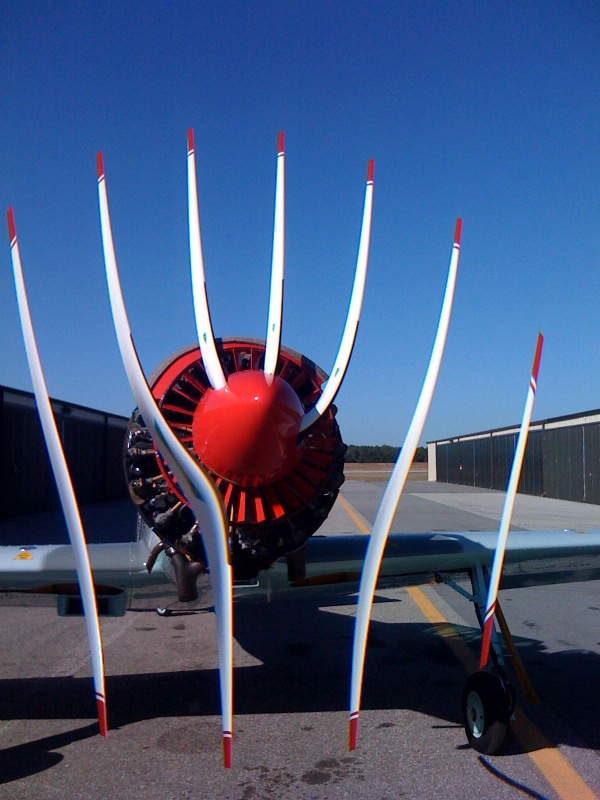
\includegraphics[scale = .25]{../tasks/kalda/rollingshutter.jpg}
		\caption{ein verzerrter Flugzeugpropeller (Bild: Soren Ragsdale, Attribution 2.0 Generic (CC BY 2.0))}
	\end{figure}\\
 Bestimme,
		\Question ob sich der Propeller mit oder gegen den Uhrzeigersinn dreht,
		\Question wie viele Flügelblätter der Propeller wirklich hat,
		\Question die Frequenz $f$ der Propellerrotation, unter der Annahme, dass die Aufnahmezeit $T=\nicefrac{1}{8}~\mathrm{s}$ betrug.
	
\end{Exercise}
\begin{Answer}[ref = rollingshutter]
	\Question Wenn man sich das Bild anschaut, stellt man fest, das in der oberen Bildhälfte mehr rote Punkte, also mehr Aufnahmen eines einzelnen Rotorblatts zu sehen sind, als in der unteren.\\
	Also kam es in der oberen Bildhälfte öfter dazu, dass sich ein Rotorblatt und der Kamerascanner an der gleichen Position befanden. Das ist aber gerade dann der Fall, wenn sich die Rotorblätter zum Kamerascanner hin bewegen.\\
	Da sich der Scanner von links nach rechts bewegt, heißt das also, dass die horizontale Geschwindigkeitskomponente der Rotorblätter von rechts nach links gerichtet ist. Also dreht sich der Propeller gegen den Uhrzeigersinn.\\
	\Question Wir 
\end{Answer}
